\section{Measurements}
\label{wosc:sec:measurements}

This section presents the measurements we made with our functions. %First, we divide the application into multiple functional categories to see how much processor time is spent in each category, then we describe and present our estimation of the function's code footprints that we use to support our findings and finally we show the top-down breakdown of microarchitectural bottlenecks and the component-wise execution performance.
For each of these measurements, we compare back-to-back and interleaved function execution and discuss the consequences.
\begin{table}
  \caption{\label{wosc:tab:timings} Percentiles of the observed running times for the functions in ms.}
  \centering
%\resizebox{0.8\columnwidth}{!}{
  % latex table generated in R 4.1.3 by xtable 1.8-4 package
% Thu Sep 29 14:52:46 2022
\begin{tabular}{lrrrr}
  \toprule
Benchmark & 50\% & 90\% & 95\% & 99\% \\ 
  \midrule
autocomplete & 0.26 & 0.29 & 0.31 & 0.38 \\ 
  deltablue & 8.82 & 9.56 & 9.65 & 15.10 \\ 
  dynamichtml & 0.47 & 0.51 & 0.54 & 0.74 \\ 
  img\_resize & 747.69 & 793.62 & 799.36 & 803.95 \\ 
  json\_dumps & 14.54 & 14.63 & 14.65 & 14.90 \\ 
  markdown\_to\_html & 38.24 & 38.43 & 38.78 & 38.92 \\ 
  ocr\_img & 1164.65 & 1177.91 & 1179.57 & 1180.89 \\ 
  sentiment\_analysis & 2.03 & 2.14 & 2.17 & 2.23 \\ 
  fib\_js\_1000 & 0.25 & 0.27 & 0.29 & 0.34 \\ 
  fib\_js\_10000 & 0.34 & 0.43 & 0.47 & 0.63 \\ 
  fib\_js\_100000 & 0.48 & 0.59 & 0.64 & 0.86 \\ 
  fib\_py\_1000 & 0.52 & 0.60 & 0.62 & 0.66 \\ 
  fib\_py\_10000 & 1.82 & 2.11 & 2.28 & 4.49 \\ 
  fib\_py\_100000 & 97.74 & 98.37 & 98.40 & 99.15 \\ 
  footprint\_long\_16 & 10.52 & 10.58 & 10.61 & 10.70 \\ 
  footprint\_long\_32 & 20.75 & 20.83 & 20.86 & 21.00 \\ 
  footprint\_long\_64 & 52.93 & 53.04 & 53.16 & 53.36 \\ 
  footprint\_long\_128 & 121.25 & 121.41 & 121.64 & 121.95 \\ 
  footprint\_long\_256 & 260.76 & 262.45 & 262.65 & 262.82 \\ 
  footprint\_short\_16 & 0.30 & 0.35 & 0.37 & 0.40 \\ 
  footprint\_short\_32 & 0.32 & 0.37 & 0.39 & 0.42 \\ 
  footprint\_short\_64 & 0.37 & 0.43 & 0.44 & 0.48 \\ 
  footprint\_short\_128 & 0.49 & 0.54 & 0.55 & 0.59 \\ 
  footprint\_short\_256 & 0.74 & 0.80 & 0.81 & 0.84 \\ 
   \bottomrule
\end{tabular}

%}
\end{table}


\begin{figure}
  \centering
  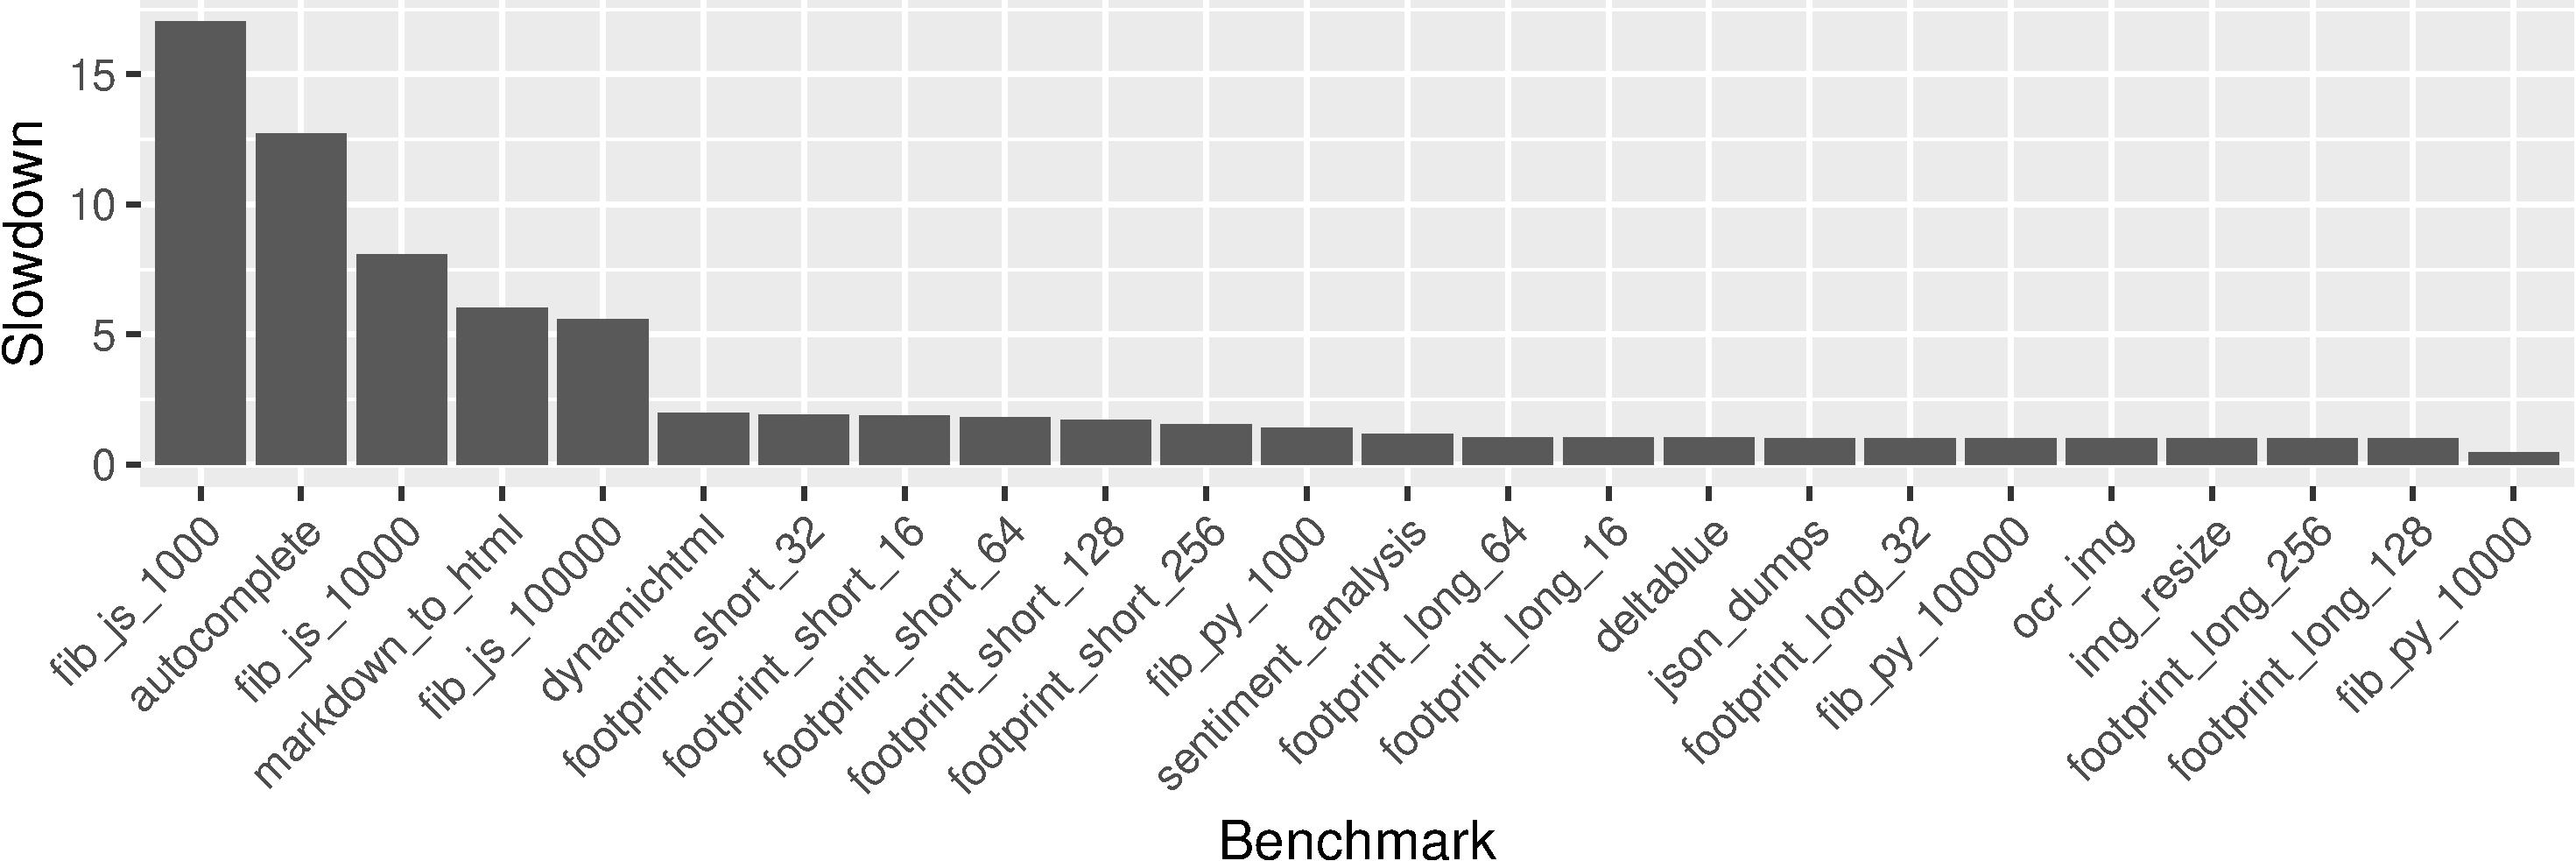
\includegraphics[width=\textwidth]{figures/thrasher_speedups.pdf}
  \caption{\label{wosc:fig:slowdown} The wall-time slowdown encountered when running functions interleaved instead of back-to-back.}
  \Description{Bar chart showing the slowdown factor the thrasher causes on individual functions.}
\end{figure}

\begin{sidewaysfigure}
  \centering
  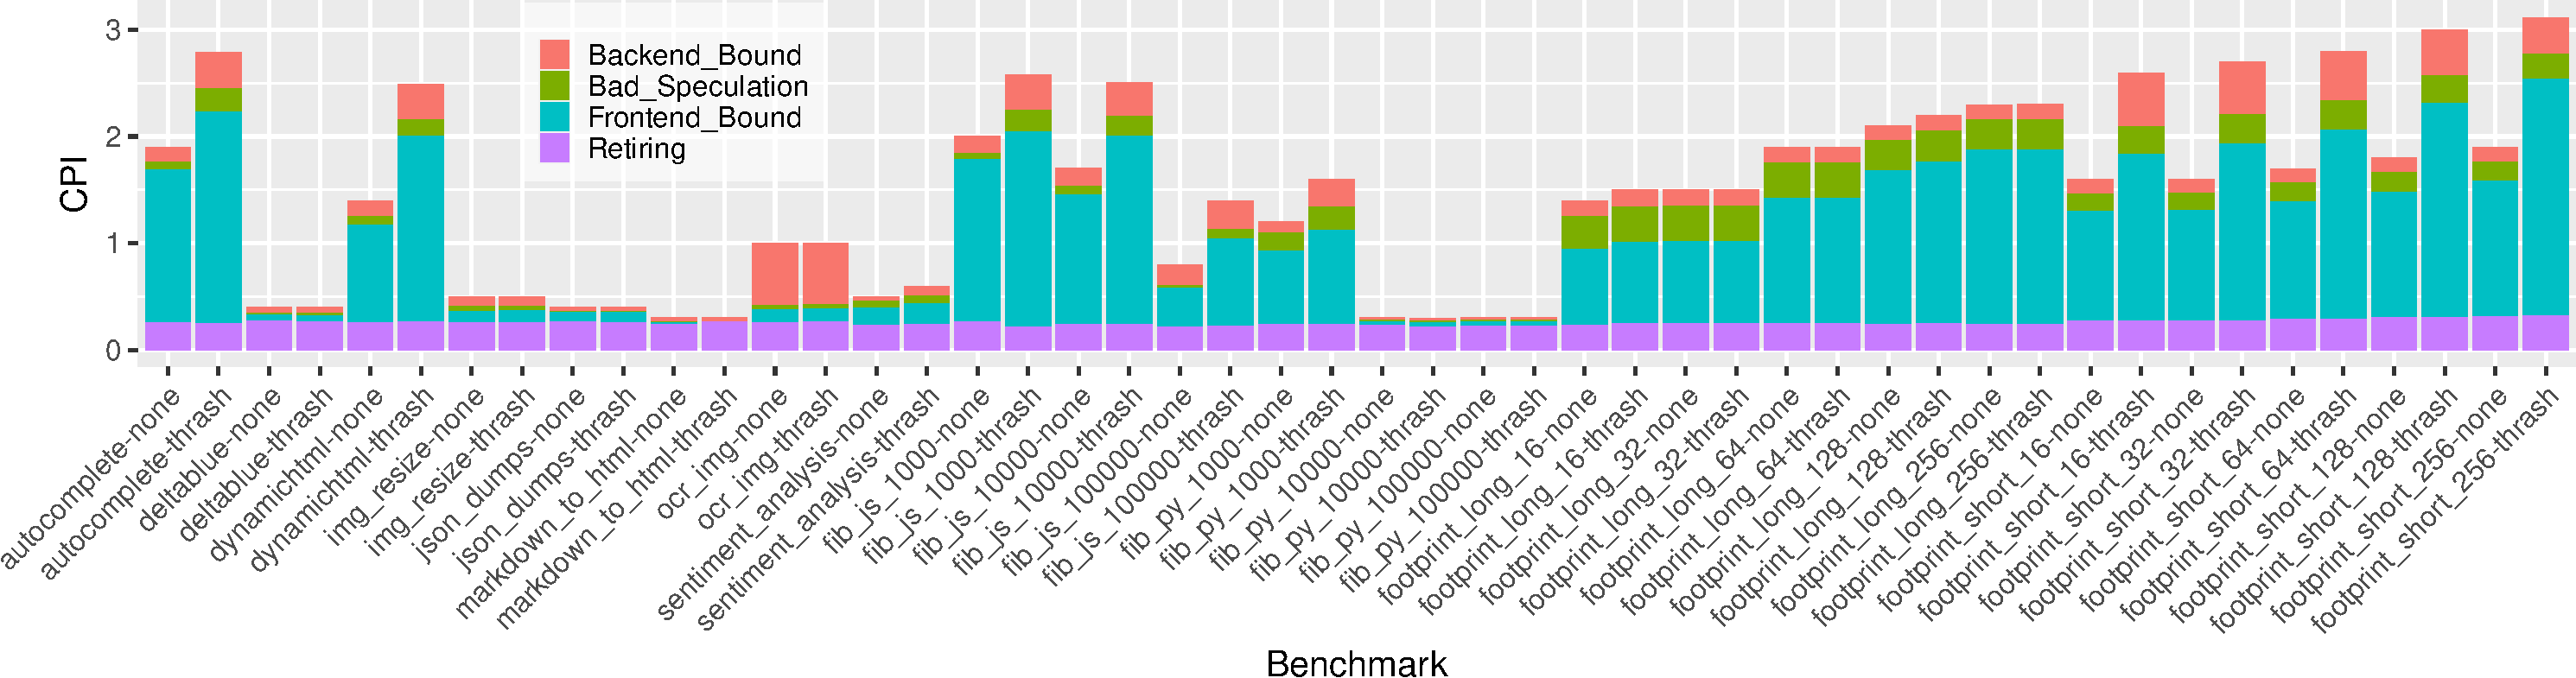
\includegraphics[width=\textwidth]{figures/topdown_level1.pdf}
  \caption{\label{wosc:fig:topdown_level1} CPI stack for the functions broken down based on the contribution from each bottleneck category.}
  \Description{Stacked bar chart showing the top-down bottlenecks for the analyzed functions.}
\end{sidewaysfigure}



\subsection{Where does time go?}
\label{wosc:subsec:time}

The invocation machinery of a FaaS function is complex and multi-layered as it involves multiple components that are not directly related to a function's core functionality. To understand the potential of these components to impact the function execution behaviour, we analyze their contribution to a request's overall processing time, \Cref{wosc:fig:cyc_per_component}. The sampled cycles are categorized primarily based on the Dynamic Shared Object (DSO, e.g. a shared library or executable) they originated from and, in some cases, secondarily subdivided based on the function that was executing when the cycle was sampled. This subdivision is necessary to correctly decompose NodeJS functions as they depend on platform-native libraries executed as JIT-generated code that do not appear as separate DSOs.

The categories shown in  \Cref{wosc:fig:cyc_per_component} were chosen to represent the majority of the execution time. They are defined as follows:
\noindent
\begin{description}
\item[Application Code]  The core part of the functionality of the function.
\item [gRPC] Cycles spent in the gRPC and Protobuf libraries.
\item [HTTP] Cycles spent processing HTTP requests.
\item [Kernel] Cycles spent in the kernel. Note that we do not trace cycles in this category back to the component that triggered their execution.
\item[Library] Cycles spent in libraries that are directly related to the core functionality of the function and only invoked from application code. For example, an image processing library is counted in this category whereas glibc is not.
\item[Linker] Cycles spent in the dynamic linker.
\item[Stdlib] Calls to C and C++ standard libraries. Like the kernel category, we do not identify who made the standard library calls.
  \end{description}

In general, application or application-specific library code dominates the CPU cycle distribution regardless of the function and execution mode used. The principal pattern that emerges is that the functions with the shortest execution times (cf. \Cref{wosc:tab:timings}) spend relatively more time in the function invocation machinery. This is not surprising considering that, unlike functions with longer execution times, they are unable to amortize the invocation overhead.

Next we look at how the cycle distribution changes when comparing back-to-back invocations of the functions to interleaved invocations. Examining this change in distribution informs us about how the various components involved in the function execution lifecycle are affected by the interference from the thrasher. If a component takes up relatively more cycles in the interleaved execution case, it means that the component is disproportionally negatively affected by the thrasher. Our results show that there are significant differences in the degree to which different functions are affected that largely depend on the function execution time. For example, in \emph{autocomplete} and \emph{dynamichtml}, which have very small execution time, we observe an increase in the fraction of cycles spent in application code with interleaved execution. In contrast, long running functions such as \emph{img\_resize} and \emph{ocr\_img} do not show much difference in cycle distribution.


Now, we demonstrate the significance of interleaved execution on functions with a short execution time from another perspective by comparing the elapsed per-invocation wall-clock time between the two invocation modes.  \Cref{wosc:fig:slowdown} shows the difference in request round trip time between back-to-back and interleaved executions as measured from the client. For the majority of the functions there is no significant difference in the execution time between the interleaved and back-to-back executions. We only see marked increases in execution time for very short functions  with < 1 ms median execution time. The most extreme example is the $17\times$ increase in execution time of the \emph{fib\_js\_1000} function.

Finally, we also observe that the execution time alone does not always explain a function's sensitivity to interleaved execution. Compare, for example, \emph{dynamichtml} to \emph{fib\_py\_1000} which have very similar execution times as depicted in \Cref{wosc:tab:timings}. For the \emph{dynamichtml} function, we see that more cycles are spent on application code in the interleaved execution case, whereas the characteristics of \emph{fib\_py\_1000} are largely unchanged. A reason for this behaviour can be that other function properties such as code and data footprints, control flow behaviour, etc. influence performance sensitivity to interleaved execution. As there can be a large number of function properties, we first analyze the ones that have the largest impact on function performance, in the next section, and then analyze the impact of thrashing on them.


\subsection{Microarchitectural analysis}
\label{wosc:subsec:topdown}

\begin{figure}
  \centering
  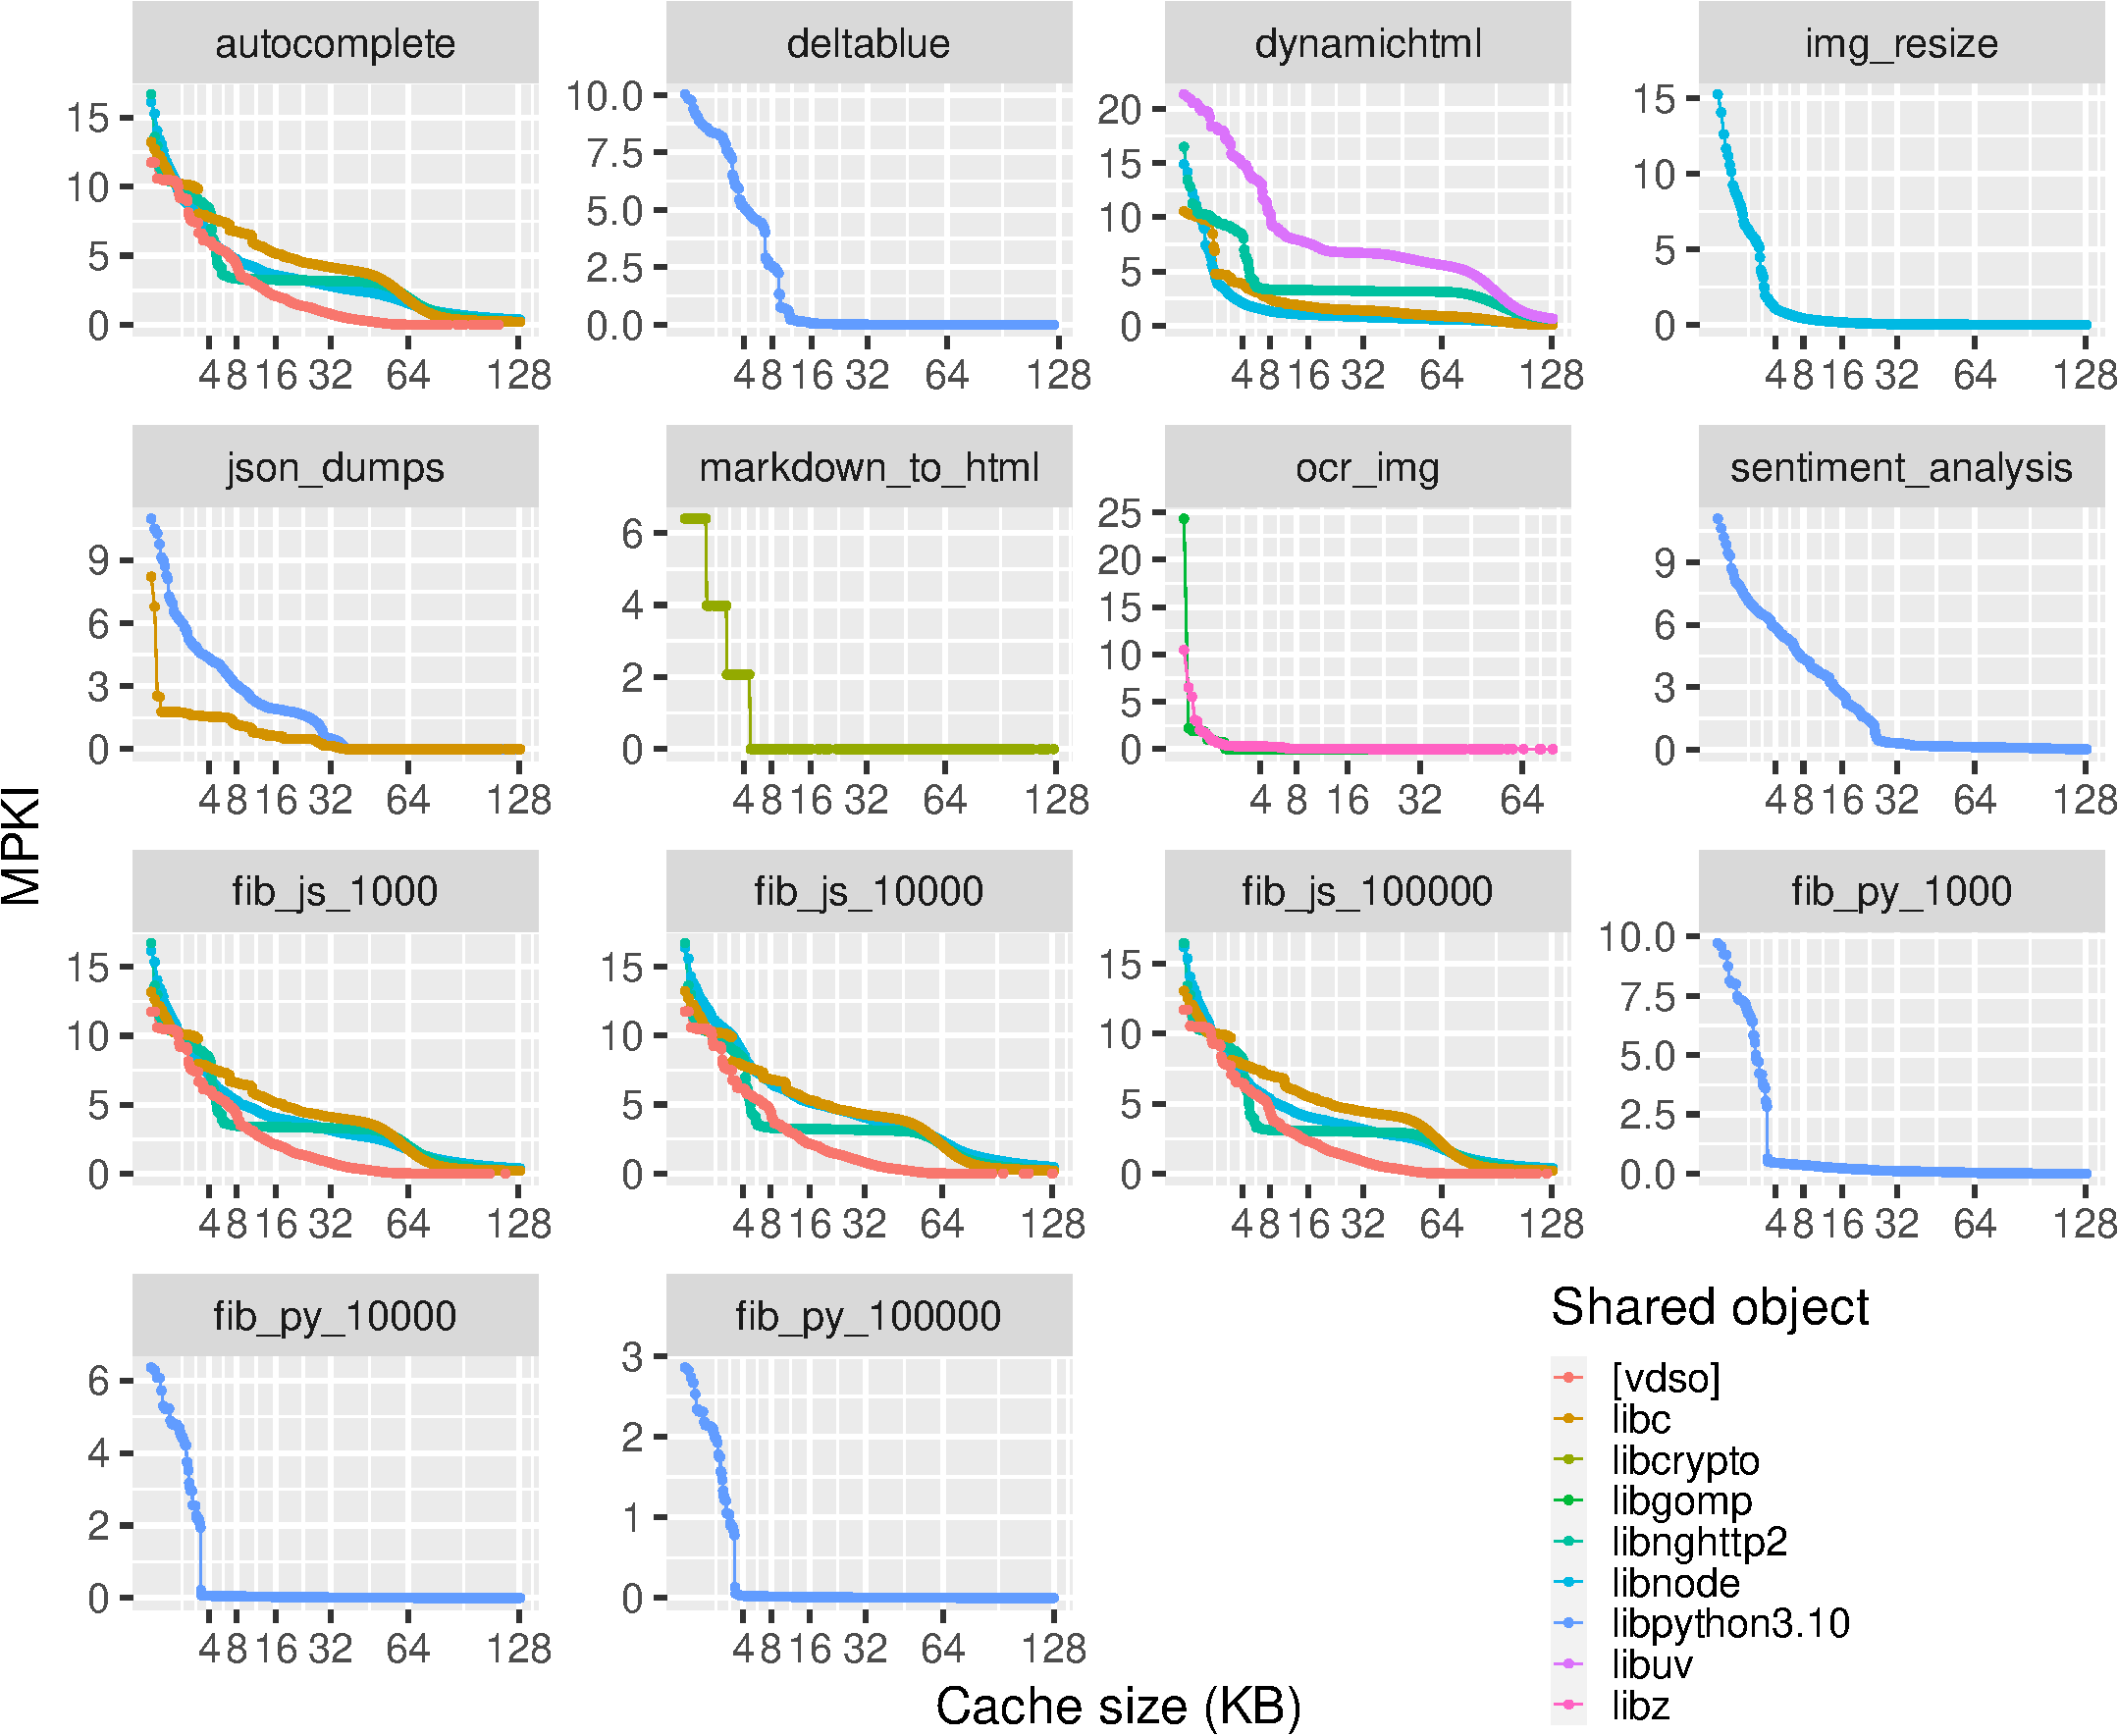
\includegraphics[width=\textwidth]{figures/simulated_miss_rates.pdf}
  \caption{\label{wosc:fig:code-footprint} The estimated instruction working set sizes of the functions.}
\end{figure}


\begin{sidewaysfigure}
  \centering
  
\includegraphics[width=\textwidth]{figures/cat-cpi.pdf}
  \caption{\label{wosc:fig:cat-cpi} The CPI for the different components of the application.}
  \Description{Bar chart showing the CPI for different parts of the application}
\end{sidewaysfigure}



To analyze the microarchitectural behaviour of our functions, we use the established Top-Down methodology \cite{yasin14_top_down}. The Top-Down methodology uses performance counters to estimate the fraction of pipeline slots that are stalled due to bottlenecks in specific parts of the processor. The top level of the analysis is broken down into four categories: \emph{Retiring}, \emph{Backend\_Bound}, \emph{Bad\_Speculation}, and \emph{Frontend\_Bound}. The \emph{Retiring} category covers slots containing retired instructions, that is, instructions that completed and committed their result. As such, this is the desirable category of Top-Down and we want to maximize the number of pipeline slots that fall in this category. \emph{Backend\_Bound} denotes slots that are stalled due to the execution units of the processor backend being unable to accept additional instructions. The \emph{Bad\_Speculation} category denotes slots that are stalled due to incorrect speculations, for example, branch mispredictions. Finally, the \emph{Frontend\_Bound} category contains slots that are stalled due to the frontend's inability to supply the backend with instructions at a sufficiently high rate. The identified bottlenecks can be broken down in a hierarchical fashion making it possible to identify a specific microarchitectural structure that is put under stress by the evaluated function.


The cycles per instruction (CPI) stacks resulting from the Top-Down analysis are shown in \Cref{wosc:fig:topdown_level1}. The CPI stack visualizes the contributions of the individual bottlenecks to the overall performance of the function. From the results, we see that there is a strong correlation between the execution time of a function and the instructions per cycle (IPC) rates that they achieve: shorter running functions achieve lower IPC rates (i.e., high CPI). Additionally, when comparing back-to-back and interleaved executions, the functions with low IPC also show the largest relative performance degradation in the interleaved execution mode. 

The figure also implies that short running functions show low IPC because of the front-end bottleneck, i.e., they are \emph{Frontend\_Bound}. These results corroborate prior work which also found serverless functions and conventional server applications to be \emph{Frontend\_Bound} and proposed diverse mechanisms to mitigate this bottleneck \cite{btbx-pact, btbx-cal, twig, shotgun, boomerang, lukewarm_serverless}. Further, prior work \cite{lukewarm_serverless} also reported that instruction cache (L1-I) misses are the principal reason for this front-end bottleneck in serverless functions. This finding suggests that the instruction working set size of the functions also has the most significant impact on their performance. To show the instruction working set of a function impacts its performance sensitivity to interleaved execution, we estimate the instruction working set of our functions in the next section.


\subsection{Estimating instruction working set}

\label{wosc:subsec:footprint}

Motivated by the Top-Down analysis results, we now estimate the instruction working set size of our functions to understand how it impacts function performance. To perform the estimation, we use a method described in  \cite{splash2} adapted to work with traces gathered using Intel PT. The result is shown in \Cref{wosc:fig:code-footprint} giving the Cumulative Distribution Functions for the functions of the estimated MPKI rate of each function's shared objects depending on the instruction cache size. When the MPKI for a cache size reaches zero, it means that the entire instruction working set of the function fits the cache. Therefore, this cache size corresponds to the instruction working set of the function. For clarity, we only show the CDFs for shared objects that combined contribute 99\% of the executed instructions or the single shared object that alone contribute more than 99\% of executed instructions.


With these results, we can now shed further light on the data presented in \Cref{wosc:subsec:time} and \Cref{wosc:subsec:topdown}. Comparing the \emph{fib\_py\_1000} and \emph{fib\_js\_10000} functions using the data from  \Cref{wosc:fig:code-footprint}, we see that the NodeJS version of the function has a significantly larger instruction working set than the Python version. The instruction working set of the Python version of the function is less than 4KB while the NodeJS implementation requires more than 64KB, a $16\times$ difference. This observed correlation remains consistent across all of the measured functions.


Next, we look at how the instruction working set of a function affects its sensitivity to interleaved execution. Looking at the synthetic footprint functions (right side of \Cref{wosc:fig:topdown_level1}) and comparing them to \emph{fib\_py\_1000} we see that, again, only functions with a short execution time are affected by interleaved execution. Additionally, for short-running functions a large instruction working set exacerbates the impact of interleaved execution. On the other hand, the performance of longer-running functions are unaffected by interleaved execution regardless of their instruction working set. The conclusion of this is that only functions with a very short execution time \emph{and} and a large instruction working set see a performance degradation because of interleaved function execution.


Finally, our results highlight the importance of choice of programming language and runtime environment for application performance.  For example, looking at \emph{fib\_js} and \emph{fib\_py} functions in \Cref{wosc:fig:topdown_level1}, the NodeJS implementation show significantly worse CPI. However, computing the 100,000th Fibonacci number takes $181\times$ longer using the Python implementation than with the NodeJS implementation as shown in \Cref{wosc:tab:timings}. This observation is far from novel but it highlights the magnitude of the gains that are possible by making purely application-level changes.


\subsection{Category-wise performance}
\label{wosc:subsec:cat-perf}



Lastly, we discuss the performance of the functions broken down by category. We divide the executed cycles into the same categories as in \Cref{wosc:subsec:time}. The results are shown in \Cref{wosc:fig:cat-cpi}. The purpose of this experiment is to assess if particular parts of the application exhibits worse performance than the average. For the back-to-back executions, no particular component diverges significantly from the average performance of the function. For the interleaved execution, a different pattern emerges. Again, only the functions with the shortest execution times are affected but the components taking the smallest part of the total execution time are disproportionally affected. For example the Linker component contributes only a negligible fraction of the executed cycles (see \Cref{wosc:fig:cyc_per_component}) of the \emph{autocomplete} function and in the back-to-back execution scenario it exhibits the same performance as the application as a whole, around 2 CPI. However, in the interleaved execution scenario, its performance deteriorates more than $2 \times$.
% Mention the relative deterioration e.g. 4x 
Meanwhile, the performance of the Application Code category deteriorates slightly, from 2 to 2.5 CPI, ending up just below the overall function performance of 2.9 CPI (as seen in \Cref{wosc:fig:topdown_level1}). The same pattern can be observed for the \emph{dynamichtml}, \emph{fib\_js\_1000} and \emph{fib\_js\_10000}
functions.


%%% Local Variables:
%%% mode: latex
%%% TeX-master: "main"
%%% End:
